\documentclass{article}

\usepackage[tmargin=.9in, bmargin=.9in, lmargin=1in, rmargin=1in]{geometry}
\usepackage{bookmark, wrapfig, enumitem, pdflscape, hyphenat}
\usepackage[labelfont=bf]{caption}
\usepackage{lmodern}
\usepackage[sfdefault]{roboto}
\usepackage[T1]{fontenc}

\usepackage{graphicx}
    \makeatletter % tex.stackexchange.com/a/28565
    \setlength{\@fptop}{0pt}
    \setlength{\@fpbot}{0pt plus 1fil}
    \makeatother

\usepackage[absolute, overlay]{textpos}
    \setlength{\TPHorizModule}{1mm}
    \setlength{\TPVertModule}{1mm}

\usepackage{xcolor}
    \definecolor{WCM}{RGB}{172,31,44} % AC1E2C

\usepackage{hyperref} \hypersetup{
    colorlinks=true, linkcolor={blue!65!black},
    citecolor={blue!65!black}, urlcolor={blue!50!black},
    pdfpagelayout=OneColumn, pdfstartview={XYZ null null 1.25},
    bookmarksnumbered=true, bookmarksopen=true, bookmarksopenlevel=3
}

\usepackage[backend=bibtex, style=nature]{biblatex}
    \addbibresource{latex/references.bib}

\newcommand{\beginsupplement}{
% bytesizebio.net/2013/03/11/adding-supplementary-tables-and-figures-in-latex
    \newpage
    \setcounter{page}{1}
    \renewcommand{\thepage}{S-\arabic{page}}
    \setcounter{table}{0}
    \renewcommand{\thetable}{S\arabic{table}}
    \setcounter{figure}{0}
    \renewcommand{\thefigure}{S\arabic{figure}}
 }

\usepackage{setspace}

\begin{document}

\begin{center}
    \Large{\textbf{Haplotype Diversity and Sequence Heterogeneity of Human Telomeres}}
    \\~\\
    \small{
        Kirill Grigorev\textsuperscript{1,2 \#},
        Jonathan Foox\textsuperscript{1,2,3 \#},
        Daniela Bezdan\textsuperscript{1,2,3},
        Daniel Butler\textsuperscript{1},
        Jared J. Luxton\textsuperscript{4,5},
        Jake Reed\textsuperscript{1},
        \\%rem
        Miles J. McKenna\textsuperscript{4,5},
        Lynn Taylor\textsuperscript{4,5},
        Kerry A. George\textsuperscript{4,5},
        Cem Meydan\textsuperscript{1,2,3},
        Susan M. Bailey\textsuperscript{4,5 *},
        Christopher E. Mason\textsuperscript{1,2,3,6 *}
    }
\end{center}

\small{ \noindent
    \textsuperscript{1} Department of Physiology and Biophysics, Weill Cornell Medicine, New York, New York, USA
    \\
    \textsuperscript{2} The HRH Prince Alwaleed Bin Talal Bin Abdulaziz Alsaud Institute for Computational Biomedicine, \\
    \textcolor{white}{\textsuperscript{2}} Weill Cornell Medicine, New York, New York, USA
    \\
    \textsuperscript{3} The Feil Family Brain and Mind Research Institute, New York, New York, USA
    \\
    \textsuperscript{4} Department of Environmental and Radiological Health Sciences, Colorado State University, Fort Collins, CO
    \\
    \textsuperscript{5} Cell and Molecular Biology Program, Colorado State University, Fort Collins, CO
    \\
    \textsuperscript{6} The WorldQuant Initiative for Quantitative Prediction, Weill Cornell Medicine, New York, NY, USA
    \\
    \textsuperscript{\#} Co-first authors
    \\
    \textsuperscript{*} Corresponding authors. Send correspondence to S.M.B. (susan.bailey@colostate.edu) \\%rem
    \textcolor{white}{\textsuperscript{*}} and C.E.M. (chm2042@med.cornell.edu)
}

\normalsize
\doublespacing

\section*{Abstract} \addcontentsline{toc}{section}{Abstract}
    Telomeres are regions of repetitive nucleotide sequences capping the ends of eukaryotic chromosomes that protect against deterioration,
        and whose lengths can be correlated with age and adverse health risk factors.
    Given their length and repetitive nature,
        telomeric regions are not easily reconstructed from short-read sequencing,
        making telomere sequence resolution a very costly and generally intractable problem.
    Recently, long-read sequencing, with read lengths measuring in hundreds of Kbp,
        has made it possible to routinely read into telomeric regions and inspect their sequence structure.
    Here, we describe a framework for
        extracting telomeric reads from whole genome single-molecule sequencing experiments,
        prior-less \textit{de novo} identification of telomere repeat motifs,
        and describing their sequence variation.
    We find that
        long telomeric stretches can be accurately captured with long-read sequencing,
        observe extensive sequence heterogeneity of human telomeres,
        discover and localize non-canonical motifs (both previously reported as well as novel),
        confirm the presence of the non-canonical motifs in short read sequencing experiments,
        and report the first motif composition maps of human telomeric haplotypes across populations on a multi-Kbp scale.

\section*{Keywords} \addcontentsline{toc}{section}{Keywords}
    Telomere, telomeric haplotypes, long-read sequencing, telomere sequence heterogeneity

\pagebreak
%\singlespacing
%\tableofcontents
\doublespacing

\section*{Introduction} \addcontentsline{toc}{section}{Introduction}
    Telomeres are the functional ends of human chromosomes that naturally shorten with cell division and therefore with age \cite{teloaging}.
    Telomere length can also be influenced by a variety of lifestyle factors and environmental exposures
        (e.g., stress, exercise, air pollution, radiation) \cite{teloeffects}.
    While human telomeres are known to consist largely of a conserved six-nucleotide repeat (TTAGGG) \cite{moyzis},
        several studies have identified variations of this motif in proximal telomeric regions
            \cite{telovars1989,telovars1999,telovars2018,telovars2019}.
    However, such studies were performed with oligonucleotide hybridization, PCR, immunoprecipitation, and short-read sequencing,
        requiring prior assumptions about specific target motifs, custom sample preparation, and targeted sequencing,
        and therefore preventing \textit{de novo} identification of motif variants and their localization.
    Thus, long-range maps of telomeric sequence variation in the human genome are still lacking.
    Such maps can provide insight into telomere biology and enable novel approaches to analyze the effects of
        health status, aging, and environment on telomere sequence and length.
    \\~\\
    To improve our understanding of telomere sequence structure and variation, we developed \textit{edgeCase},
        a framework for alignment and \textit{de novo} telomeric motif discovery
        which uses human whole genome long-read sequencing experiments,
            making it easily scalable.
    We have validated these methods using
        Genome in a Bottle \cite{giab} single-molecule real-time (SMRT) sequencing datasets
            generated with Pacific Biosciences circular consensus sequencing (PacBio CCS) \cite{pacbio,pacbioccs},
        and short-read Illumina \cite{illumina} and 10X Genomics (Chromium) \cite{10x} datasets.
    These results provide evidence for
        multiple novel, non-canonical telomeric repeats,
        resolution of multiple chromosome-specific haplotypes with SMRT sequencing,
        and a new method for long-range characterization of the structure of telomeric sequences.

\section*{Results} \addcontentsline{toc}{section}{Results}

\subsection*{A telomere-annotated reference genome enables recovery of telomeric reads from human long-read whole genome sequencing datasets}
\addcontentsline{toc}{subsection}{A telomere-annotated reference genome enables recovery of telomeric reads from human long-read whole genome sequencing datasets}
    We constructed an extended reference genome, \textit{hg38ext},
        that combines chromosome sequences of the \textit{hg38} reference genome \cite{grch38,hg38}
            and human subtelomeric assemblies \cite{riethman2014},
        resulting in a reference set annotated with boundaries of subtelomeric and telomeric tracts.
            % (see \hyperref[sec:methods]{Materials and Methods}).
        The layout of this reference set is available in \textbf{Supplemental File S1},
            and the set itself can be reproduced with a script available as \textbf{Supplemental File S2}.
    We then aligned PacBio CCS reads of seven Genome in a Bottle (GIAB, \cite{giab}) human subjects (HG001 through HG007) to \textit{hg38ext},
        and in total, observed reads mapping to the ends of chromosomes and extending into telomeric regions
            on 10 \textit{p} arms and 19 \textit{q} arms,
                with 53\textendash{}295 such reads on the \textit{p} arms
                and 384\textendash{}1119 on the \textit{q} arms
                    (\textbf{Supplemental Table S1}).
    Portions of reads contained in the telomeric regions were extracted for further analysis (\textbf{\autoref{fig:schematic_alignment}}).
        \begin{figure}[h!] \centering % \vspace{5mm}
        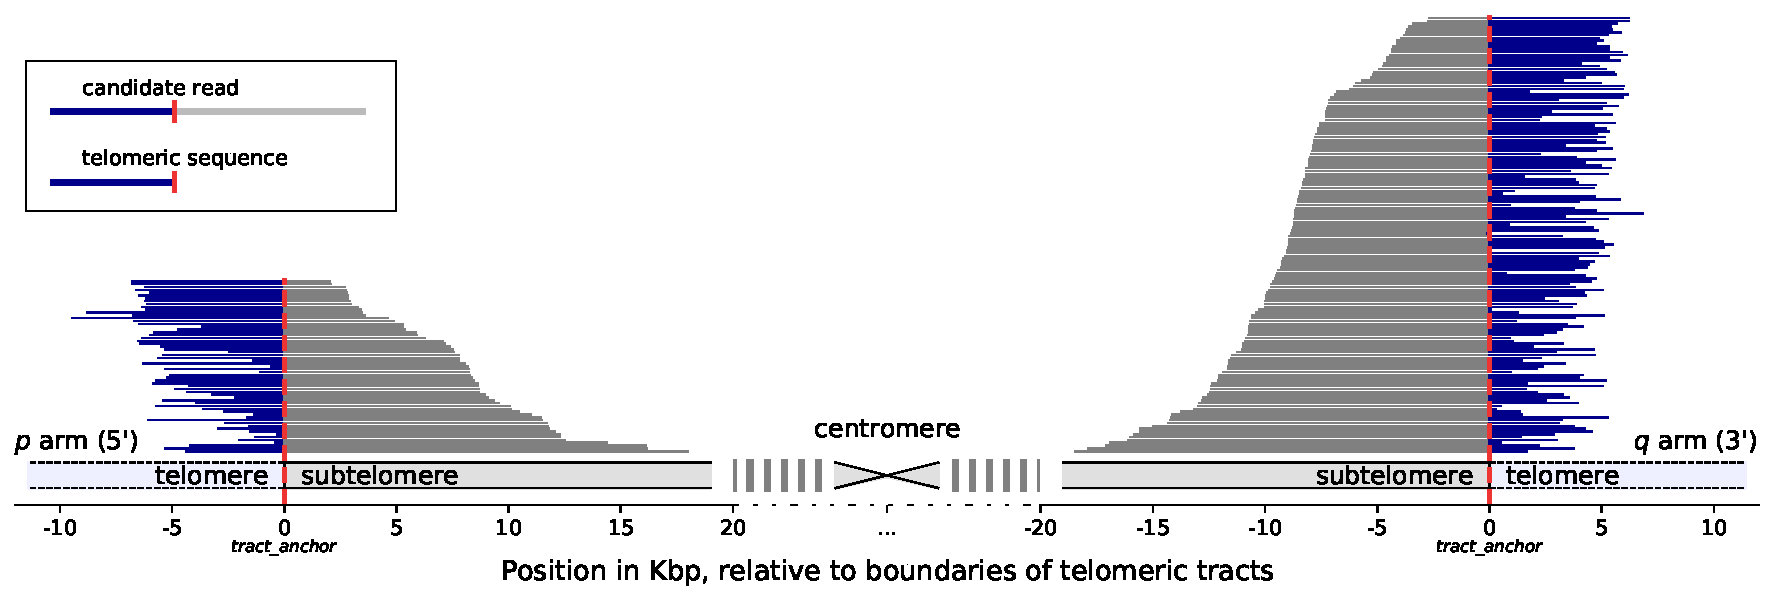
\includegraphics[height=.75\textheight,width=\textwidth,keepaspectratio]{renders/figures/Figure-1.pdf}
        \caption{
             \small Mapping of candidate telomeric reads, illustrated with reads from the HG002 dataset aligning to \mbox{chromosome 5.}
             The chromosome is displayed schematically, centered around the centromere.
             Vertical red dashed lines denote the position of the boundary of the annotated telomeric tract.
             Coordinates are given in Kbp, relative to the positions of the telomeric tract boundaries.
             Statistics for all chromosomes of all seven datasets are provided in \textbf{Supplemental Table S1}.
        }
        \label{fig:schematic_alignment}
        \end{figure}

\subsection*{Telomeric long reads contain variations of the canonical motif}
\addcontentsline{toc}{subsection}{Telomeric long reads contain variations of the canonical motif}
    We performed \textit{de novo} repeat discovery in the telomeric sequences for motifs of lengths 4 through 16,
            and identified motifs in repeat contexts that are statistically enriched in the seven datasets.
        The majority of motifs were either the canonical TTAGGG / CCCTAA,
            its variations (e.g., TT\underline{G}GGG / CCC\underline{C}AA),
            or a duplet of variants, such as TTAGGGTTA\underline{G}GGG
            (\textbf{\autoref{tab:repeatfinder}}).
        CG-rich motifs were also observed on the \textit{p} arms.
        The top enriched motif (TTAGGG / CCCTAA) explained
            62.2\%\textendash{}82.5\% of the telomeric repeat content on the \textit{q} arms
            and 11.6\%\textendash{}36.3\% on the \textit{p} arms,
            and three more motifs (TT\underline{G}GGG, TTA\underline{G}GGG, T\underline{G}AGGG)
                each explained at least 1\% of the repeat content in all seven datasets.
    \\~\\
    We visualized the locations of the top four enriched motifs and their reverse complements
        on the chromosomal ends of the HG002 dataset (\textbf{\autoref{fig:hg002_densityplot}}),
        as it provided the deepest coverage among the assessed datasets (\textbf{Supplemental Table S1}).
        Only the chromosomal arms covered by at least 25 reads were plotted.
            Plots for the other six datasets are available as \textbf{Supplemental Figs. S1\textendash{}S6}.
        \begin{landscape} \begin{samepage} \begin{table}[h!] \scriptsize \begin{tabular}{lllllllllllllllll}
\hline
\textbf{Arm} & \textbf{Motif} & \multicolumn{7}{l}{\textbf{Percentage of sequence explainable by motif, \%}} & \multicolumn{7}{l}{\textbf{Score}} & \textbf{Combined adjusted} \\
\textbf{}    & \textbf{}      & \textbf{HG001} & \textbf{HG002} & \textbf{HG003} & \textbf{HG004} & \textbf{HG005} & \textbf{HG006} & \textbf{HG007} &   \textbf{HG001} &   \textbf{HG002} &   \textbf{HG003} &   \textbf{HG004} &   \textbf{HG005} &   \textbf{HG006} &   \textbf{HG007} &  \textbf{p value} \\
\hline
q            &         TTAGGG & 74.5  & 82.5  & 80.1  & 81.7  & 75.7  & 77.5  & 62.2  &  0.6295 &  0.7126 &  0.6255 &  0.6497 &  0.6113 &  0.5988 &  0.4550 &  9.51e-113 \\
\textbf{}    &         TTGGGG &  2.5  &  3.4  &  2.8  &  2.8  &  2.4  &  3.1  &  6.6  &  0.0158 &  0.0229 &  0.0175 &  0.0179 &  0.0155 &  0.0197 &  0.0434 &   4.04e-58 \\
\textbf{}    &        TTAGGGG &  4.6  &  4.8  &  7.2  &  6.0  &  5.1  &  7.6  &  9.0  &  0.0152 &  0.0166 &  0.0200 &  0.0163 &  0.0161 &  0.0232 &  0.0279 &  4.22e-110 \\
\textbf{}    &         TGAGGG &  1.9  &  2.5  &  1.7  &  2.0  &  3.6  &  2.9  &  4.1  &  0.0128 &  0.0162 &  0.0102 &  0.0129 &  0.0230 &  0.0184 &  0.0265 &   1.15e-47 \\
\textbf{}    &         TTCGGG &  1.2  &  0.5  &  0.7  &  0.4  &  1.4  &  1.1  &  2.5  &  0.0080 &  0.0034 &  0.0043 &  0.0025 &  0.0095 &  0.0077 &  0.0168 &   7.68e-46 \\
\textbf{}    &  TTAGGGTTAGGGG &  3.0  &  3.3  &  6.3  &  5.4  &  3.7  &  6.0  &  6.5  &  0.0043 &  0.0050 &  0.0090 &  0.0073 &  0.0053 &  0.0083 &  0.0092 &  2.76e-102 \\
\textbf{}    &         TCAGGG &  0.9  &  0.7  &  1.1  &  1.0  &  1.1  &  0.8  &  1.4  &  0.0065 &  0.0044 &  0.0078 &  0.0069 &  0.0082 &  0.0058 &  0.0087 &   1.22e-24 \\
\textbf{}    &          TTAGG &  1.8  &  1.6  &  3.4  &  4.2  &  2.0  &  3.2  &  1.9  &  0.0048 &  0.0041 &  0.0092 &  0.0110 &  0.0052 &  0.0084 &  0.0049 &   4.60e-94 \\
\textbf{}    &          TAGGG &  2.3  &  1.9  &  3.1  &  3.0  &  2.8  &  3.2  &  2.4  &  0.0050 &  0.0039 &  0.0067 &  0.0063 &  0.0058 &  0.0067 &  0.0048 &   5.75e-91 \\
\textbf{}    &    TTAGGTTAGGG &  2.7  &  2.6  &  5.2  &  6.5  &  2.8  &  4.9  &  2.5  &  0.0037 &  0.0034 &  0.0069 &  0.0088 &  0.0037 &  0.0065 &  0.0033 &   1.97e-89 \\
\textbf{}    &         TAGGGC &  0.5  &  0.4  &  0.6  &  0.6  &  0.8  &  0.2  &  1.3  &  0.0039 &  0.0032 &  0.0047 &  0.0047 &  0.0060 &  0.0014 &  0.0099 &   5.64e-42 \\
\textbf{}    &        TTTAGGG &  1.5  &  1.5  &  1.4  &  1.4  &  1.4  &  2.2  &  2.5  &  0.0048 &  0.0039 &  0.0029 &  0.0028 &  0.0034 &  0.0055 &  0.0058 &   2.32e-79 \\
\textbf{}    &         TAGGGG &  0.7  &  0.9  &  0.6  &  0.9  &  0.7  &  0.6  &  1.2  &  0.0035 &  0.0051 &  0.0028 &  0.0044 &  0.0034 &  0.0025 &  0.0060 &   2.68e-42 \\
\textbf{}    &    TAGGGTTAGGG &  3.1  &  2.6  &  3.9  &  4.0  &  3.5  &  3.8  &  2.9  &  0.0036 &  0.0031 &  0.0041 &  0.0041 &  0.0041 &  0.0040 &  0.0035 &   1.45e-84 \\
\textbf{}    &        TTAAGGG &  0.8  &  1.2  &  1.1  &  0.8  &  1.0  &  1.2  &  1.3  &  0.0022 &  0.0030 &  0.0032 &  0.0021 &  0.0029 &  0.0034 &  0.0032 &   4.87e-70 \\
\textbf{}    &          TTGGG &  1.4  &  0.9  &  1.9  &  1.7  &  1.8  &  1.9  &  1.4  &  0.0022 &  0.0013 &  0.0032 &  0.0026 &  0.0028 &  0.0028 &  0.0022 &   3.17e-70 \\
\textbf{}    &  TTAGGGTTTAGGG &  1.2  &  1.4  &  1.4  &  1.5  &  1.3  &  2.0  &  2.3  &  0.0011 &  0.0017 &  0.0013 &  0.0014 &  0.0016 &  0.0021 &  0.0033 &   5.17e-68 \\
\textbf{}    &    TTGGGTTAGGG &  1.7  &  1.0  &  2.1  &  1.9  &  1.9  &  2.0  &  1.1  &  0.0012 &  0.0007 &  0.0013 &  0.0014 &  0.0015 &  0.0014 &  0.0008 &   1.75e-53 \\
\textbf{}    &  TTAGGGTTAAGGG &  0.5  &  1.0  &  0.9  &  0.5  &  0.7  &  0.7  &  1.0  &  0.0005 &  0.0020 &  0.0009 &  0.0004 &  0.0006 &  0.0009 &  0.0007 &   1.03e-50 \\
p            &         CCCTAA & 21.5  & 36.3  & 19.9  & 17.1  & 32.0  & 16.9  & 11.6  &  0.1687 &  0.3113 &  0.1491 &  0.1258 &  0.2639 &  0.1255 &  0.0831 &  9.51e-113 \\
\textbf{}    &         CCCCAA &  1.5  &  1.6  &  1.4  &  1.1  &  1.8  &  1.1  &  1.4  &  0.0100 &  0.0104 &  0.0087 &  0.0073 &  0.0120 &  0.0073 &  0.0093 &   1.05e-73 \\
\textbf{}    &        CCCCTAA &  2.3  &  2.4  &  1.9  &  2.0  &  2.2  &  1.9  &  1.9  &  0.0075 &  0.0075 &  0.0054 &  0.0059 &  0.0067 &  0.0056 &  0.0061 &  9.17e-109 \\
\textbf{}    &         CCCTCA &  0.2  &  0.6  &  0.5  &  0.5  &  0.4  &  0.6  &  0.5  &  0.0009 &  0.0044 &  0.0033 &  0.0029 &  0.0025 &  0.0037 &  0.0035 &   1.05e-50 \\
\textbf{}    &  CCCCTAACCCTAA &  1.8  &  2.0  &  1.6  &  1.6  &  2.0  &  1.6  &  1.3  &  0.0029 &  0.0031 &  0.0023 &  0.0023 &  0.0029 &  0.0023 &  0.0022 &   1.46e-97 \\
\textbf{}    &         GGCGCA &  2.1  &  1.8  &  1.4  &  1.1  &  1.6  &  1.4  &  1.1  &  0.0028 &  0.0023 &  0.0019 &  0.0014 &  0.0022 &  0.0020 &  0.0016 &   2.35e-27 \\
\textbf{}    &          CCGCG &  1.1  &  0.8  &  0.7  &  0.5  &  0.8  &  0.9  &  0.9  &  0.0028 &  0.0020 &  0.0018 &  0.0013 &  0.0021 &  0.0022 &  0.0021 &  4.35e-100 \\
\textbf{}    &          CCCTA &  0.9  &  1.1  &  1.0  &  0.9  &  1.2  &  0.8  &  0.5  &  0.0020 &  0.0021 &  0.0022 &  0.0019 &  0.0026 &  0.0015 &  0.0010 &   2.38e-98 \\
\textbf{}    &          CCTAA &  0.8  &  1.0  &  0.9  &  0.9  &  0.6  &  0.6  &  0.4  &  0.0020 &  0.0026 &  0.0023 &  0.0023 &  0.0016 &  0.0016 &  0.0010 &  5.75e-100 \\
\textbf{}    &    CCCTAACCTAA &  1.1  &  1.6  &  1.3  &  1.2  &  0.9  &  0.9  &  0.5  &  0.0015 &  0.0021 &  0.0017 &  0.0016 &  0.0012 &  0.0012 &  0.0007 &   1.47e-80 \\
\textbf{}    &    CCCTACCCTAA &  1.1  &  1.3  &  1.2  &  0.9  &  1.6  &  0.9  &  0.5  &  0.0012 &  0.0020 &  0.0012 &  0.0011 &  0.0021 &  0.0010 &  0.0007 &   6.67e-77 \\
\hline
\end{tabular}
\caption{
    \small Significantly enriched repeating motifs in telomeric regions of GIAB datasets HG001 through HG007.
    Only the motifs that explain at least 1\% of the telomeric sequence on either arm of at least one dataset,
    with respect to reverse-complemented equivalence, are included.
    See \hyperref[sec:methods]{Materials and Methods} for the definition of \textit{score}.
}
\label{tab:repeatfinder}
\end{table}
\end{samepage}
\end{landscape}
 % tab:repeatfinder
        \begin{figure}[h!] \centering
        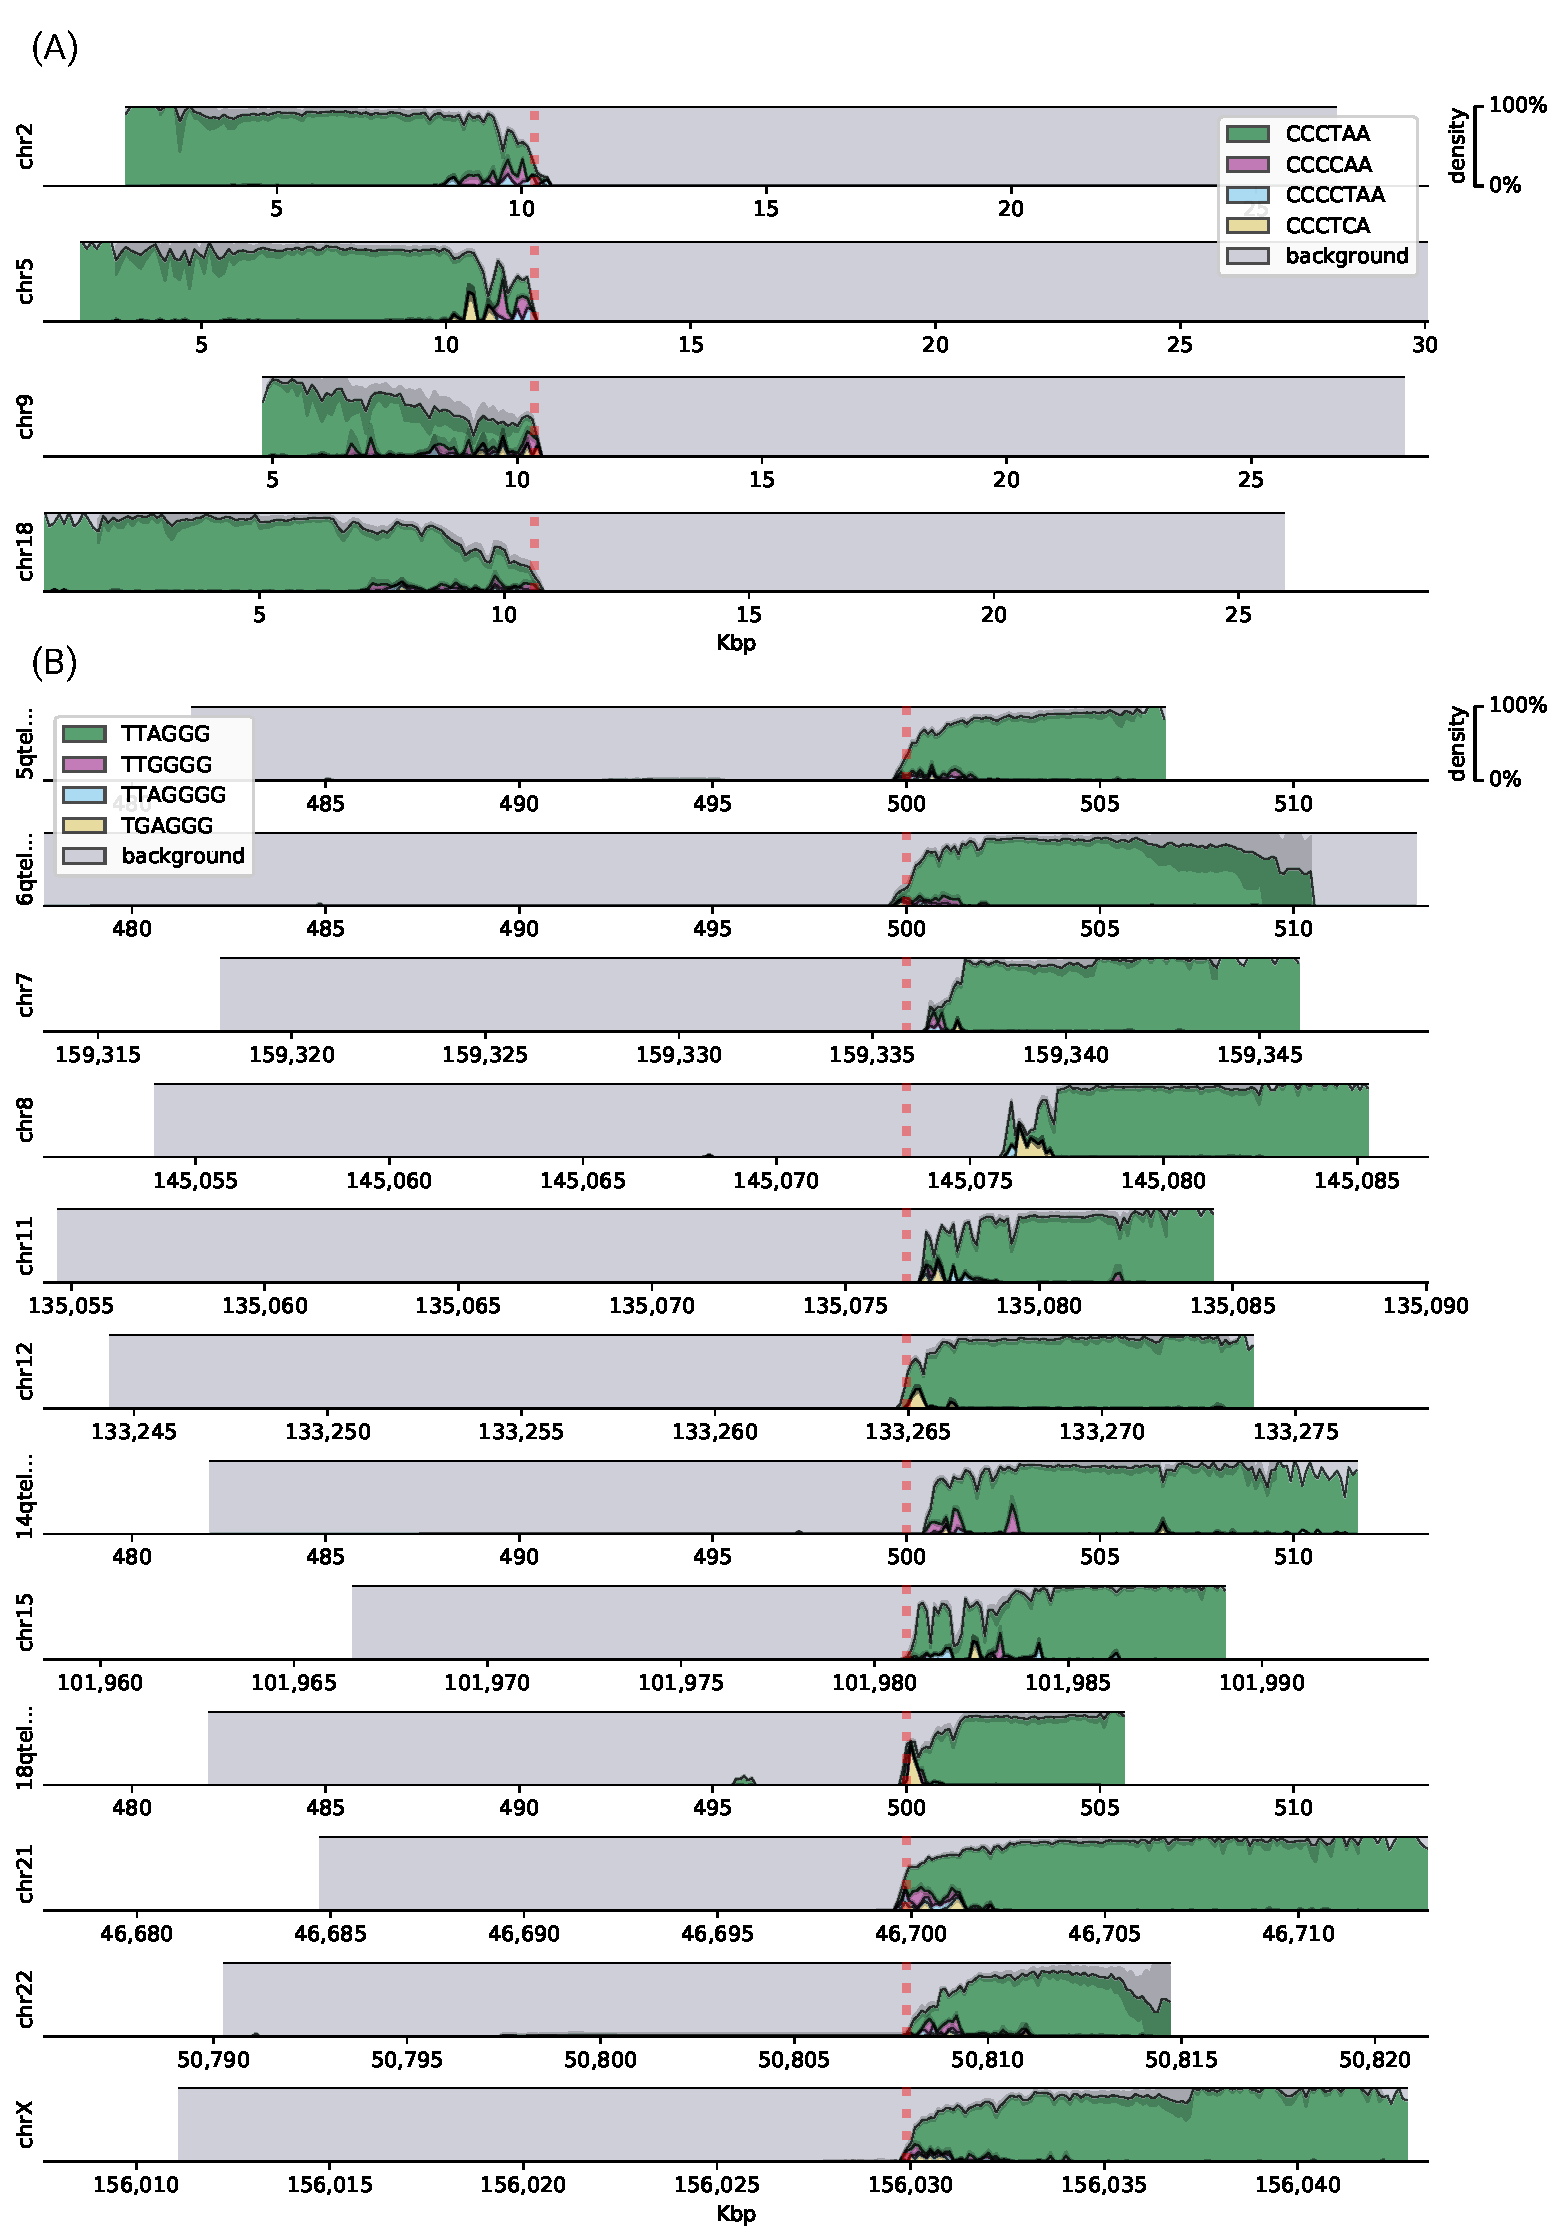
\includegraphics[height=.88\textheight,width=\textwidth,keepaspectratio]{renders/figures/Figure-2.pdf}
        \caption{
             \small Densities of the top four enriched motifs at ends of chromosomal \textbf{(A)} \textit{p} arms
             and \textbf{(B)} \textit{q} arms of the HG002 dataset.
             \textit{Background} represents the remaining sequence content (non-repeating sequence and not significantly enriched motifs).
             Only the arms covered by at least 25 reads are displayed.
             Reads are shown aligned to the contigs in the \textit{hg38ext} reference set, and genomic coordinates are given in Kbp.
             Vertical red dashed lines denote the position of the boundary of the annotated telomeric tract.
        }
        \label{fig:hg002_densityplot}
        \end{figure}
    \noindent % \\~\\
    Long reads on each arm agreed on the locations of different motifs within any given 10 bp window
        (the coverage-weighted median of normalized Shannon entropy was 0.00 for all data,
        and the coverage-weighted 3rd quartile was 0.00\textendash{}0.13,
        \textbf{\autoref{fig:entropy}}),
        indicating that locations of the variations are colinear among reads.
        \begin{figure}[h!] \centering
        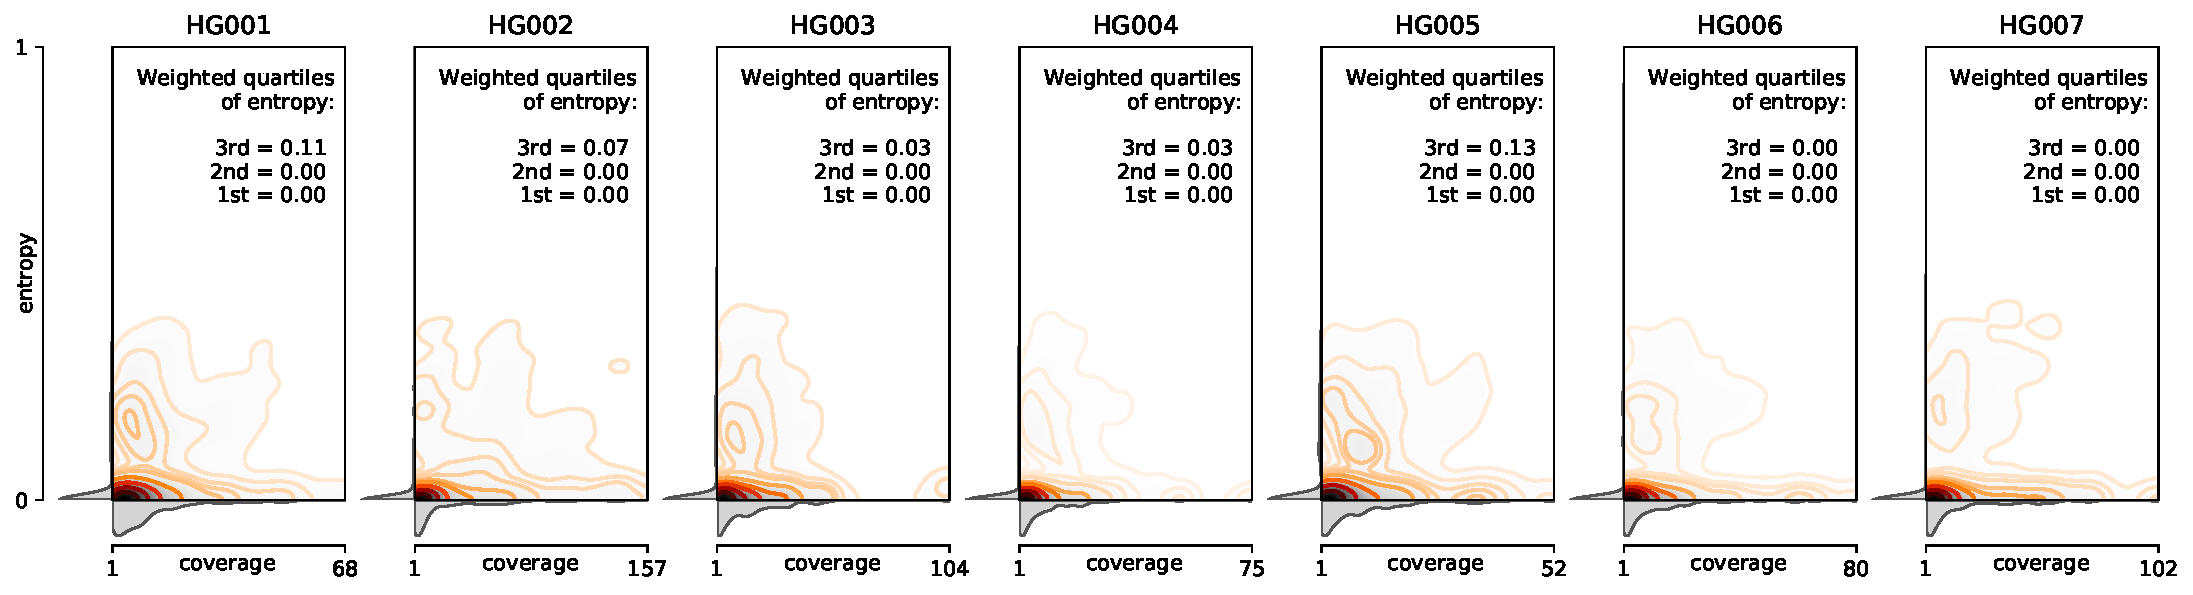
\includegraphics[height=.75\textheight,width=\textwidth,keepaspectratio]{renders/figures/Figure-3.pdf}
        \caption{
            \small Distribution of motif entropies in 10 bp windows of of candidate PacBio CCS reads aligning to the same chromosomal arms
            in GIAB datasets HG001 through HG007,
            with respect to per-window coverage,
            and the coverage-weighted quartiles of the entropy values.
            % no fourth quartile: https://math.stackexchange.com/a/1468111
        }
        \label{fig:entropy}
        \end{figure}

\subsection*{Short-read sequencing validates motif variations observed in long reads}
\addcontentsline{toc}{subsection}{Short-read sequencing validates motif variations observed in long reads}
    We validated these findings using short-read sequencing in two ways.
    First, we found that telomeric candidate reads extracted with \textit{Telomerecat} \cite{telomerecat}
        from respective GIAB Illumina datasets
        supported a definitive majority of the telomeric sequence on the \textit{q} arms of long-read datasets
            (median 98\% of the sequence supported, \textbf{Supplemental Fig. S7}).
        At the same time, only a median of 38\% of the sequence of the \textit{p} arm long reads was supported,
            and while this does not automatically invalidate them (see \hyperref[sec:discussion]{Discussion}),
            only the long reads mapping to the \textit{q} arms were used for downstream analyses.
    Second, we confirmed 15 of the enriched motifs in independently generated human short-read and linked-read genomic datasets,
        with the same four motifs being the most enriched (\textbf{Supplemental Table S2}).

\subsection*{Long-read sequencing uncovers a variety of human telomeric haplotypes}
\addcontentsline{toc}{subsection}{Long-read sequencing uncovers a variety of human telomeric haplotypes}
    While reads agreed on colinearity of motifs, evidenced by low entropy,
        rarer non-zero entropy values could be attributable both to sequencing errors
        and to structural variations within the same subject's dataset.
    To investigate the latter possibility,
        we clustered reads on each \textit{q} arm of each subject by relative pairwise Levenshtein distances \cite{levenshtein}
        and found that hierarchical clustering described read similarity well,
            resulting in high cophenetic correlation between the dendrograms and the pairwise distance matrices
                (\textbf{\autoref{tab:cophenetic}}),
            and in visible structure (\textbf{\autoref{fig:haplotypes}}).
            % \eject \pdfpageheight=40in \pdfpagewidth=22in
                \begin{figure}[h!] \centering % \vspace{5mm}
                \includegraphics[height=.88\textheight,width=\textwidth,keepaspectratio]{renders/figures/Figure-4.png}
                \caption{
                    \small Clustering of reads by relative pairwise Levenshtein distances (unitless measure)
                    on each chromosomal \mbox{\textit{q} arm} of datasets HG001 through HG007,
                    and densities of top four enriched motifs along each read.
                    Each horizontal line represents an individual read;
                    Genomic coordinates are given in Kbp, relative to the positions of the telomeric tract boundaries.
                    Only the chromosomal arms cumulatively covered by at least 25 reads are displayed.
                }
                \label{fig:haplotypes}
                \end{figure}
            % \eject \pdfpageheight=11in \pdfpagewidth=8.5in
            \begin{samepage} \begin{table}[h!] \small \begin{tabular}{llll}
\hline
\textbf{Chromosome} & \textbf{Reference contig}       & \multicolumn{2}{l}{\textbf{Cophenetic correlation}} \\
\textbf{}           & \textbf{}                       & \textbf{r} & \textbf{p}                             \\
\hline
chr5                & 5qtel\_1-500K\_1\_12\_12\_rc    & 0.491      & <1.0e-300                              \\
chr6                & 6qtel\_1-500K\_1\_12\_12\_rc    & 0.366      & <1.0e-300                              \\
chr7                & chr7                            & 0.683      & <1.0e-300                              \\
chr8                & chr8                            & 0.273      & <1.0e-300                              \\
chr11               & chr11                           & 0.435      & <1.0e-300                              \\
chr12               & chr12                           & 0.395      & <1.0e-300                              \\
chr14               & 14qtel\_1-500K\_1\_12\_12\_rc   & 0.620      & <1.0e-300                              \\
chr15               & chr15                           & 0.457      & <1.0e-300                              \\
chr16               & 16qtel\_1-500K\_1\_12\_12\_rc   & 0.747      & 7.82e-79                               \\
chr18               & 18qtel\_1-500K\_1\_12\_12\_rc   & 0.520      & <1.0e-300                              \\
chr19               & chr19                           & 0.520      & 2.40e-294                              \\
chr21               & chr21                           & 0.388      & <1.0e-300                              \\
chr22               & chr22                           & 0.568      & <1.0e-300                              \\
chrX                & chrX                            & 0.453      & <1.0e-300                              \\
\hline
\end{tabular}
\caption{
    \small Measures of cophenetic correlation (Pearson's \textit{r} and adjusted \textit{p}-value)
    between the hierarchical clustering and the pairwise distance matrix
    on each chromosomal \textit{q} arm.
}
\label{tab:cophenetic}
\end{table}
\end{samepage}
 % tab:cophenetic
    ~\\~\\
    In this complex clustering, subject- and population-specific variation was evident and quantifiable via relative Levenshtein distances
        (\textbf{\autoref{tab:haptests}}; see \hyperref[sec:methods]{Materials and Methods}):
        overall,
            telomeric reads within a subject were more similar than within a population
                (adjusted Wilcoxon signed-rank test \textit{p} = 7.7e-223),
            and telomeric reads within a population were more similar than between populations
                (\textit{p} = 3.1e-120).
        ~\\
        \begin{samepage} \begin{table}[h!] \small \begin{tabular}{ll}
\hline
\textbf{Comparison}                                                                     & \textbf{Adjusted p-value} \\
\hline
A subject's reads are closer to each other than to other subjects' reads in the trio    & 7.7e-223                  \\
A subject's reads are closer to each other than to subjects' reads in other populations & <1.0e-300                 \\
Reads within a population are closer to each other than to reads in other populations   & 3.1e-120                  \\
Ashkenazim trio:                                                                        & \textbf{}                 \\
\hspace{.5cm} Father's reads are closer to son's reads than to mother's reads           & 9.5e-33                   \\
\hspace{.5cm} Mother's reads are closer to son's reads than to father's reads           & 1.9e-26                   \\
Chinese trio:                                                                           & \textbf{}                 \\
\hspace{.5cm} Father's reads are closer to son's reads than to mother's reads           & \textit{ns}               \\
\hspace{.5cm} Mother's reads are closer to son's reads than to father's reads           & \textit{ns}               \\
\hline
\end{tabular}
\caption{
    \small Adjusted \textit{p}-values of the Wilcoxon signed-rank tests on relative Levenshtein distances.
    For each read, closest distances to groups of reads described in the \textit{Comparison} column are compared
    (see \hyperref[sec:methods]{Materials and Methods}).
}
\label{tab:haptests}
\end{table}
\end{samepage}

        ~\\
        Importantly, however, this was true for most, but not all reads;
            4\% of all assessed reads (142 out of 3,686) contributed to interpopulation similarity;
                these reads were twice as close to reads from a different population than they were to any reads of their own subjects.
            (Another 388 reads, or 11\%, also clustered away from their respective subjects, but by a less than 2x distance ratio).
            This trend is observable on \textbf{\autoref{fig:haplotypes}},
                with subjects' and populations' reads interspersed across multiple clusters.
        Therefore, the captured reads reflected spectra of haplotypes,
            generally describing subject- and population-specific similarities,
            but including a sizable component that described interpopulation similarity.
        Familial inheritance of variation was also observed:
            either parent's telomeric reads were more similar to their son's than to the other parent's reads in the Azhkenazim trio.
            In the Chinese trio,
                the amount of inheritance of variation from either parent to the son was not found to be statistically significant overall,
                but was present on several of the assessed chromosomes (\textbf{Supplemental Table S3}).

\section*{Discussion} \addcontentsline{toc}{section}{Discussion} \label{sec:discussion}
    Repeat-rich, low-complexity regions of the human genome such as telomeres
        have been historically recalcitrant to full mapping and annotation \cite{miga2015},
        mainly due to the alignment challenge they pose and to the read lengths required to span such areas \cite{ngslowcomplexity}.
    The advent of long-read, single-molecule methods (third generation sequencing)
        has provided new opportunities to map the sequence composition of a previously "dark" area of the human genome,
        enabling research into the sequence composition and length dynamics \cite{luxton2020} of telomeres.
    Our results reaffirm
        that the canonical repeat (TTAGGG) is certainly the most dominant type of motif in telomeres,
        but also reveal a surprising diversity of repeat variations,
            which are confirmed by both short and long-read sequencing technologies.
    This diversity of repeats includes previously reported variants,
        as well as novel motifs that are characterized not only by nucleotide substitutions,
        but also insertions, deletions, and even motif pairing.
    Apart from these variations,
        CG-rich motifs were identified in telomeric regions of \textit{p} arms,
        consistent with previously reported findings \cite{cpg}.
    Moreover, while short read sequencing is able to identify such variants,
        it alone cannot reveal the relative locations of these motifs within telomeres,
        as repetitive short reads can
            neither be aligned outside of the reference genome
            nor provide enough overlap variability to be assembled \textit{de novo}.
    Long SMRT reads, on the other hand,
        can be anchored to known subtelomeric sequences of the human genome and extend into the previously unmapped telomeric area.
    Furthermore, in contrast to previously published research that utilized targeted sequencing
        \cite{telovars1989,telovars1999,telovars2018,telovars2019},
        the method described here allows identification of multiple enriched motifs and their localization
            \textit{de novo}, without any bias introduced by prior knowledge about the sequence of target motifs.
    These results also highlight the need of better subtelomeric and telomeric annotations in the human genome:
    Four of the 40 subtelomeric assemblies \cite{riethman2014}
        were homologous to regions in the reference genome far within the respective chromosomes (up to 586 Kbp into the reference sequence),
        and the canonical motif was present on the \textit{q} arm of chr8
            only after 2\textendash{}3Kbp past the annotated boundary in all datasets,
        suggesting that the existing assemblies do not provide a completely accurate telomeric annotation,
        and that methods described herein could help to resolve these areas of reference genomes.
    \\~\\
    We observed PacBio CCS reads reaching up to 16 Kbp beyond the known regions of the genome,
        and resolving the underlying sequence with reasonable fidelity,
        measured both by the entropy of motif assignment and by pairwise Levenshtein distances
            between the reads belonging to the same chromosomal arms.
    While short reads also provided support for non-canonical motifs,
        the overlap between the short and the long reads was substantial, but not complete,
        which can be explained by the necessary bias towards the canonical motif during the selection of short reads.
    Therefore, telomeric regions with higher content of non-canonical repeats are less likely to be identified through the use of short reads,
        and instead, long reads appear to be more suitable for this purpose as well.
    Of note, the captured PacBio CCS reads that mapped to \textit{q} arm telomeres
        agreed with short read sequences much better (median 98\% support, \textbf{Supplemental Fig. S7})
        than the reads that mapped to \textit{p} arm telomeres (median 38\% support).
        While, for this reason, we opted to choose only the \textit{q} arm reads for deeper analysis,
            this discrepancy can lend itself to multiple potential explanations,
                from artifacts of SMRT technology preventing faithful reproduction of the sequence,
                to the inherent bias of short-read based methods \cite{telomerecat} towards the canonical motif CCCTAA
                    that in fact could be present at a lower percentage on \textit{p} arm telomeres.
            Therefore, more research is required to determine the level of deviation of \textit{p} arm telomeric sequences
                from those on \textit{q} arms, and into biases and limitations of different technologies
                    for sequencing distal \textit{p} arm chromosomal regions.
    \\~\\
    The identified variations in long range contexts elucidate
        subject-specific, trio- and population-specific similarities of \textit{q} arm telomeric sequences,
            as well as a level of interpopulation similarity,
        and thus provide a new means of haplotype mapping and reveal the existence and motif composition of haplotype spectra
            on a multi-Kbp scale.
    Interpopulation similarity, as well as familial inheritance of variation in the Ashkenazim trio,
        evidenced that the observed haplotypes could not be attributed to per-dataset batch effects.
    Coverage of different chromosomes was uneven,
        and as such, numbers of captured telomeric reads and levels of observed similarity varied from chromosome to chromosome;
        this calls for more sequencing experiments aimed to reconstruct the full picture of this variation.
    Clustering on a per-subject basis concealed interpopulation similarity,
        but underscored intra-subject variation (\textbf{Supplemental Fig. S8}),
            suggesting coexistence of multiple telomeric haplotypes per \textit{q} arm within each subject.
        Given that the reference DNA for the subjects HG001 through HG007
            was extracted from growths of B lymphoblastoid cell lines,
            this suggests that as B cells undergo maturation,
                distinct clones may gain distinct variations in their telomeric sequence.
        This opens up avenues of investigation into the haplotypic variation among not only immune cells,
            but also different cell types overall.
%TODO for reviewers: stress that the shift from diplotypes to spectra does not invalidate the previous findings: we were able to put these findings and the method into a broader context and see more structure.

\section*{Materials and Methods} \addcontentsline{toc}{section}{Materials and Methods} \label{sec:methods}

\subsection*{The extended reference genome}
\addcontentsline{toc}{subsection}{The extended reference genome}
    We constructed the extended reference genome by performing an all-to-all alignment
        of all contigs in the \textit{hg38} reference genome \cite{grch38,hg38}
        and the subtelomeric assemblies \cite{riethman2014}
        with \textit{minimap2} \cite{minimap} using three settings
            for assembly-to-reference mapping (\textit{asm5}, \textit{asm10}, \textit{asm20}).
    Forty subtelomeric contigs mapped to ends of \textit{hg38} chromosomes with a mapping quality of 60,
        one (XpYptel) mapped with the quality of 0 and was discarded;
        one (14qtel) mapped to the ALT version of chr14 (chr14\_KI270846v1\_alt) with the quality of 52,
            which, in turn, mapped to the main chr14 chromosome with the quality of 60.
    These data and the exact match and mismatch coordinates were used to create a combined reference (\textit{hg38ext})
        in which subtelomeric contigs informed the locations of the boundaries of the telomeric tracts (\textit{tract\_anchor}).
    Such contigs that mapped fully within \textit{hg38} chromosomes resulted in \textit{tract\_anchor} annotations
            directly on those \textit{hg38} chromosomes;
        partially mapping contigs were considered as forking from the \textit{hg38} sequence and were similarly annotated by themselves.

\subsection*{Detection of telomeric sequences in long-read datasets}
\addcontentsline{toc}{subsection}{Detection of telomeric sequences in long-read datasets}
    Seven subjects were selected for the analysis.
    The first individual (NA12878/HG001) came from the pilot genome of the HapMap project \cite{HG001},
    while the other six,
        including
            the Ashkenazim Jewish Trio (son: NA24385/HG002, father: NA24149/HG003, mother: NA24143/HG004)
            and the Chinese Trio \\%rem
            (\mbox{son: NA24631/HG005}, father: NA24694/HG006, mother: NA24695/HG007),
        are members of the Personal Genome Project,
            whose genomes are consented for commercial redistribution and reidentification \cite{HG00X}.
    These subjects are referred to hereafter as HG001 through HG007, respectively.
    \\~\\
    Multiple Genome in a Bottle \cite{giab} PacBio CCS \cite{pacbio,pacbioccs} datasets were available and combined per each subject,
        with mean coverages of individual datasets ranging from $\sim$21x to $\sim$69x (\textbf{Supplemental Table S4}).
    Reads were mapped to \textit{hg38ext} with \textit{minimap2},
        and reads that mapped to either end of either chromosome and overlapped the boundary of its telomeric tract
        were selected for further analysis (\textbf{\autoref{fig:schematic_alignment}}).
    These reads had a portion of their sequence mapped to the reference contig and a portion extending beyond the reference
        (soft- or hard-clipped in the alignment file).
    Sequences past the \textit{tract\_anchor} marker were extracted from the reads that had this marker within their mapped portion
        (from the 5' end to the marker on \textit{p} arms and from the marker to the 3' end on \textit{q} arms,
        accounting for forward and reverse mappings).

\subsection*{Evaluation of telomeric content in short- and linked-read datasets}
\addcontentsline{toc}{subsection}{Evaluation of telomeric content in short- and linked-read datasets}
    To evaluate the concordance of telomeric reads captured by long- and short-read technologies,
        we extracted candidate telomeric reads from GIAB Illumina datasets for each subject (\textbf{Supplemental Table S4})
            with \textit{Telomerecat} \cite{telomerecat},
            and mapped the short reads back onto the candidate long reads from the same subject's dataset with \textit{minimap2},
            allowing all secondary mappings.
        Then, we calculated the fractions of each long read that was supported by the short reads that aligned to it.
    \\~\\
    To evaluate sequence motifs in independent samples collected from human subjects (as opposed to reference cell lines),
        we generated four whole-genome Illumina datasets (mean coverage $\sim$104x)
        and three linked-read 10X datasets (mean coverage $\sim$28x) for one individual at different timepoints,
        and one additional linked-read 10X dataset (coverage $\sim$47x) for another individual.
    These data were originally obtained from astronaut subjects for an unrelated space biology experiment,
        and the blood samples were collected from the subjects as described in \cite{twins_study}.
        For each sample, 1.2ng of sorted immune cell input was aliquoted for
            TruSeq PCR-free WGS (short read) and standard Chromium 10X whole genome (linked-read) preparation respectively,
            and sequenced across one S4 flow cell on an Illumina NovaSeq 6000.
    From these datasets, candidate telomeric short reads were selected using Telomerecat \cite{telomerecat}.

\subsection*{Identification of repeat content}
\addcontentsline{toc}{subsection}{Identification of repeat content}
    Overrepresentation of motifs of lengths $k \subset [4 .. 16]$ was tested within the candidate telomeric regions of PacBio CCS reads,
        as well as in the candidate reads from independently generated Illumina and 10X Chromium datasets.
    To target motifs in repeat contexts,
        doubled sequences (for example, \textit{k}-mer ACGTACGT for motif ACGT) were counted with \textit{jellyfish} \cite{jellyfish},
        and counts of \textit{k}-mers synonymous with respect to circular shifts (for example, ACGTACGT and CGTACGTA) were summed together.
    For each such \textit{k}-mer,
        Fisher's exact test was performed to determine whether its count is significant
            on the background of counts of other \textit{k}-mers of the same length.
    Briefly, we considered \textit{k}-mers with counts higher than 1.5 interquartile range above the third quartile of the distribution
        as potentially classifiable,
        and a $ 2 \times{} 2 $ contingency matrix $ C $ for the test was constructed as follows:
        row 0 contained counts of potentially classifiable \textit{k}-mers,
        row 1 contained counts of remaining (non-classifiable) \textit{k}-mers,
        columns 0 and 1 contained counts of single and remaining (background) \textit{k}-mers, respectively,
            i.e.:
                $ C_{0,0} = $ {\rmfamily count of target \textit{k}-mer},
                $ C_{0,1} = $ {\rmfamily sum of counts of other potentially classifiable \textit{k}-mers},
                $ C_{1,0} = $ {\rmfamily median count of \textit{k}-mer},
                $ C_{1,1} = $ {\rmfamily sum of counts of other non-classifiable \textit{k}-mers}.
    The resultant \textit{p}-values for each motif among the samples were combined using the Mudholkar-George method \cite{george}
        within each technology (PacBio CCS, Illumina, 10X Genomics),
        and the Bonferroni multiple testing correction was applied.
    Motifs in the long-read datasets for which \textit{k}-mers yielded \textit{p}-values below the cutoff of 0.05 were reported.
    As even doubled sequences (such as ACGTACGT for motif ACGT) can partially overlap at the boundaries of repeat contexts,
        we quantified their presence in the telomeric reads in two distinct ways.
        Consider a sequence such as TTAGGG(\underline{TTAGTTAG})GGTTA:
            the inner (TTAG)x2 repeat can be explained by the repeats of the canonical motif extending into it from either side;
            the middle part of a similar sequence with a bigger number of the repeats of the 4-mer, TTAGGG\underline{TTAG(TTAGTTAG)TTAG}GGTTA,
                can only be explained by the repeats of said 4-mer.
        On the one hand, the maximum fraction of the sequence that can be explained by any one motif is a useful metric,
            and it was calculated and reported.
        On the other hand, the fraction of the \textit{k}-mers attributable to a specific motif \textendash{} and not to any others \textendash{}
            elucidates the extent of deviation from the background repeat context,
            and identifies motifs that most affect the sequence structure;
            it was calculated as well and reported as each motif's score.
    Additionally, motifs that were significantly enriched in the datasets produced by all three technologies (PacBio, Illumina, 10X),
        with respect to reverse-complemented equivalence, were reported.

\subsection*{Evaluation of sequence concordance in telomeric long reads}
\addcontentsline{toc}{subsection}{Evaluation of sequence concordance in telomeric long reads}
    As telomeric reads contain long low-complexity regions and present an alignment challenge,
        we evaluated concordance of their sequences without realignment of their portions that extended past the reference sequence.
    To that end, for all reads mapping to the same chromosomal arm,
        we calculated densities of each identified motif in a rolling window starting from the innermost mapped position of each entire read.
    To evaluate whether the reads on the same arm agree on the positions of different motifs,
        for each read, we calculated motif densities in 10 bp windows with 10 bp smoothing to buffer insertions and deletions.
    For each window in each read,
        the motif with the highest density was selected to represent that window.
    Then, normalized Shannon entropy among all reads was calculated in each window as $ S = \frac{ - \sum_{i} \; ( p_{i} ln p_{i} )}{ln N} $,
        where $ p_{i} $ is the frequency of each motif in the window and $ N $ is the number of motifs \cite{hepc_entropy}.
    The value of normalized entropy was a metric bounded by $ [ 0, 1 ] $,
        with $ 0 $ describing perfect agreement and $ 1 $ describing maximum randomness.
    For motif visualization,
        we performed 1000 rounds of bootstrap of the calculated density values in the 10 bp rolling windows,
            and selected the lower and the upper bounds of the 95\% confidence interval of bootstrap.
    Of note, several chromosome arms had the \textit{tract\_anchor} position further away from the end of the contig than others
            ($\sim$79\textendash{}586 Kbp into the chromosome sequence),
        and the reads mapping to these arms did not contain these motifs,
        suggesting that
            either their subtelomeric annotations were incorrect
            or large insertions or duplications were present in the reference genome;
        in light of this, reads mapping to
            the \mbox{\textit{p} arm} of chr1,
            the \textit{q} arm of chr4,
            and both arms of chr20
        were removed from the study,
        and the analysis was repeated.

\subsection*{Identification of telomeric haplotypic variation}
\addcontentsline{toc}{subsection}{Identification of telomeric haplotypic variation}
    Within groups of reads mapping to each \textit{q} arm, all relative pairwise Levenshtein distances were calculated.
    In short, Levenshtein distance is a string metric defined as the edit distance between two strings (sequences),
        equal to the minimum number of single-character insertions, deletions, and substitutions
            required to make these sequences identical \cite{levenshtein}.
    For each pair of reads, this metric was calculated and represented absolute edit distance;
        the relative distance was then computed as the absolute distance divided by the length of the overlap,
            to normalize for the variation of such lengths.
    Pairwise relative distances were then clustered using Ward's method via the Euclidean metric,
        resulting in hierarchical structure describing the extents of similarity among reads.
    To quantify how accurately hierarchical clustering described this similarity,
        cophenetic distances \cite{cophenetic} between the hierarchies (dendrograms) and the distance matrices was calculated,
        and their Pearson correlation coefficients and Bonferroni-corrected \textit{p}-values were reported.
    \\~\\
    We then traversed the distance matrices,
        and for each read, tracked the closest reads by category:
            closest reads from the same subject,
            from the same trio (population),
            and from the outgroup (other populations).
        For the Ashkenazim and the Chinese trios, we also tracked the closest reads
            between the parents
            and between each parent and the child.
        Thus, for each read, we determined whether it locally clustered
            within its own category
                (for example, with other reads of the same subject, or with other reads from the same population)
            or in a different one
                (for example, with other reads of a different population),
            and the value of the distances that drove either clustering.
        Performing the Wilcoxon signed-rank test on these values between either categories
            provided us with \textit{p}-values that, after a Bonferroni correction,
            described whether reads tended to cluster in their own category or in a different one.
        Additionally, we also identified the minority of reads that did not follow the overall trend,
            and quantified the extent to which they did so
                (such as the reads that contributed to interpopulation similarity).

\section*{Data access} \addcontentsline{toc}{section}{Data access}
The NASA Life Sciences Data Archive (LSDA) is the repository for all human and animal research data, including the whole genome Illumina and 10X Chromium sequencing datasets from subjects aboard the ISS that were used in this study.
These datasets are protected by the terms of the Weill Cornell Medicine Internal Review Board (IRB) and can be made available to be shared upon request.
LSDA has a public facing portal where data requests can be initiated (\href{https://lsda.jsc.nasa.gov/Request/dataRequestFAQ}{lsda.jsc.nasa.gov/Request/dataRequestFAQ});
the LSDA team provides the appropriate processes, tools, and secure infrastructure for archival of experimental data and dissemination while complying with applicable rules, regulations, policies, and procedures governing the management and archival of sensitive data and information.
The LSDA team enables data and information dissemination to the public or to authorized personnel either by providing public access to information or via an approved request process for information and data from the LSDA in accordance with NASA Human Research Program and JSC Institutional Review Board direction.
\\~\\
%\section*{Availability and implementation} \addcontentsline{toc}{section}{Availability and implementation}
The software for identification of telomeric reads, \textit{de novo} discovery of repeat motifs, haplotype inference and motif density visualization was implemented in Python and is freely available at \\%rem
\href{https://github.com/lankycyril/edgecase}{github.com/lankycyril/edgecase}.

\section*{Acknowledgements} \addcontentsline{toc}{section}{Acknowledgements}
We would like to thank
the Epigenomics Core Facility at Weill Cornell Medicine,
the Scientific Computing Unit (SCU),
XSEDE Supercomputing Resources,
as well as
the STARR grants I9-A9-071, I13-0052,
The Vallee Foundation,
The WorldQuant Foundation,
The Pershing Square Sohn Cancer Research Alliance,
NASA (NNX14AH51G, NNX14AB02G, NNX17AB26G),
The National Institutes of Health (R01MH117406, \\%rem
R01NS076465, R01CA249054, R01AI151059, P01HD067244, P01CA214274),
TRISH (NNX16AO69A:0107, \\%rem
NNX16AO69A:0061),
the LLS (9238-16, Mak, MCL-982, Chen-Kiang),
and
the NSF (1840275).

\section*{Author contributions} \addcontentsline{toc}{section}{Author contributions}
S.M.B. and C.E.M. conceived the study.
K.G., J.F., and C.E.M. developed the framework and analyzed the data.
D.Bu., J.J.L., M.J.M., L.T., and K.A.G. participated in collection and processing of the ISS samples.
D.Be., D.Bu., J.J.L, J.R., and C.M. analyzed the data.
All authors edited the manuscript.

\section*{Competing interests} \addcontentsline{toc}{section}{Competing interests}
The authors declare no relevant conflict of interest, although C.E.M. is a Co-Founder of Onegevity.

\section*{References} \addcontentsline{toc}{section}{References}
\begingroup \raggedright \singlespacing \printbibliography[heading=none] \endgroup

\end{document}
